\documentclass[11pt,a4paper]{article}
\usepackage[utf8]{inputenc}
\usepackage[T1]{fontenc}
\usepackage{amsmath,amssymb,amsfonts}
\usepackage{geometry}
\geometry{top=2.2cm, bottom=2.2cm, left=2.2cm, right=2.2cm}
\usepackage{booktabs}
\usepackage{array}
\usepackage{xcolor}
\usepackage{fancyhdr}
\usepackage{hyperref}
\usepackage{enumitem}
\usepackage{tcolorbox}
\usepackage{tabularx}
\usepackage{graphicx}

\renewcommand{\tablename}{Tabla}
\renewcommand{\figurename}{Figura}
\renewcommand{\abstractname}{Resumen}

\definecolor{primary}{RGB}{18, 52, 86}
\definecolor{secondary}{RGB}{41, 128, 185}
\definecolor{darkgray}{RGB}{50, 50, 50}
\definecolor{boxbg}{RGB}{245, 248, 252}
\definecolor{boxframe}{RGB}{41, 128, 185}

\hypersetup{colorlinks=true, linkcolor=secondary, citecolor=secondary, urlcolor=secondary}

\pagestyle{fancy}
\fancyhf{}
\fancyhead[L]{\small \textcolor{darkgray}{Reporte Final del Proyecto - Aprendizaje por Refuerzo - Team 29}}
\fancyhead[R]{\small \textcolor{darkgray}{\today}}
\fancyfoot[C]{\thepage}
\renewcommand{\headrulewidth}{0.5pt}

\title{\vspace{-1.4cm}\textbf{\LARGE \textcolor{primary}{Reporte Final del Proyecto del Curso}}\\[0.25cm]
\Large \textcolor{secondary}{Navegación Autónoma con \(Q\)-Learning Tabular en un\\Entorno Dinámico de Cuadrícula \(8 \times 8\) con Obstáculos Móviles}}

\author{\textbf{\tt\small Team 29}\\
{\tt\small \textbf{Silvio Yopasa Romero} \qquad \textbf{Edgar Andrés Pérez Mora}}\\
{\tt\small \{s.yopasa, ea.perezm1\}@uniandes.edu.co}\\
\small Maestría en Inteligencia Artificial (MAIA)\\
\small Universidad de los Andes}

\date{\today}

\begin{document}
\maketitle
\thispagestyle{fancy}
\hrule \vspace{0.3cm}

\begin{abstract}
Este documento presenta el reporte final del proyecto de Aprendizaje por Refuerzo sobre navegación autónoma en una cuadrícula de \(8 \times 8\). El agente debe desplazarse desde \((0,0)\) hasta \((7,7)\) evitando cinco obstáculos móviles que se trasladan de forma simultánea en cada paso de tiempo. Se formalizan los componentes del Proceso de Decisión de Markov (MDP) estados completos, representación perceptual reducida, acciones, recompensas y transición— junto con los ajustes implementados respecto a la entrega parcial anterior. Adicionalmente, se detallan el entorno de ejecución, los tiempos de entrenamiento, el almacenamiento de la \(Q\)-tabla y los resultados de evaluación sobre \(500\) y \(1{,}000\) episodios, contrastando los comportamientos esperados con las limitaciones observadas durante las pruebas.
\end{abstract}

\vspace{0.25cm} \hrule \vspace{0.35cm}

\section{Definición del Ambiente, Estados, Acciones, Recompensas y Cambios Realizados}

\subsection{Descripción del ambiente y estado completo (\(\mathcal{S}\))}
El entorno consiste en un cuarto cerrado de \(8 \times 8\) casillas indexadas por fila \(x \in \{0,\dots,7\}\) y columna \(y \in \{0,\dots,7\}\). El agente inicia siempre en la esquina superior izquierda \((0,0)\) con orientación aleatoria \(\theta_0 \in \{\text{Este } (1), \text{Sur } (2)\}\), y su objetivo es alcanzar la esquina inferior derecha \((7,7)\). Cinco obstáculos móviles se inicializan aleatoriamente en casillas distintas de \((7,7)\) que cumplen una distancia Manhattan segura \(\ge 3\) respecto a \((0,0)\).

Para satisfacer la propiedad de Markov en el ambiente completo, el estado en el instante \(t\) está compuesto por la posición y orientación del agente junto con las coordenadas de los cinco obstáculos:
\begin{equation}
    s_t = \big(x_a, y_a, \theta_a, (x_{o_1}, y_{o_1}), (x_{o_2}, y_{o_2}), (x_{o_3}, y_{o_3}), (x_{o_4}, y_{o_4}), (x_{o_5}, y_{o_5})\big)
\end{equation}
donde \(\theta_a \in \{0=\text{Norte}, 1=\text{Este}, 2=\text{Sur}, 3=\text{Oeste}\}\). El episodio finaliza cuando el agente alcanza un estado terminal:
\begin{itemize}[leftmargin=1.2cm]
    \item \textbf{Éxito (\(\mathcal{S}_{\text{meta}}\)):} \((x_a, y_a) = (7, 7)\).
    \item \textbf{Colisión (\(\mathcal{S}_{\text{colisión}}\)):} \(\exists\, i \in \{1,\dots,5\}\) tal que \((x'_a, y'_a) = (x'_{o_i}, y'_{o_i})\) o cruce frontal simultáneo en la arista intermedia \(\big((x'_a, y'_a) = (x_{o_i}, y_{o_i}) \land (x'_{o_i}, y'_{o_i}) = (x_a, y_a)\big)\).
\end{itemize}

\subsection{Representación perceptual reducida y cambios desde la última entrega}
Dado que el espacio de estados completo tiene cardinalidad \(|\mathcal{S}| = 8 \times 8 \times 4 \times 64^5 \approx 2.75 \times 10^{11}\), se utiliza una representación perceptual egocéntrica para indexar la \(Q\)-tabla. Respecto a la entrega anterior, se realizaron las siguientes modificaciones para incrementar la capacidad de evasión bajo movimientos simultáneos:

\begin{enumerate}[leftmargin=1.2cm]
    \item \textbf{Ampliación de sensores frontales y laterales de 2 a 3 niveles (\(\{0, 1, 2\}\)):}
    En la entrega previa, los sensores \(\text{obs}_{\text{frente}}, \text{obs}_{\text{izq}}, \text{obs}_{\text{der}} \in \{0, 1\}\) solo detectaban si la casilla adyacente estaba ocupada en el instante \(t\). Sin embargo, como los obstáculos se mueven \emph{al mismo tiempo} que el agente, un obstáculo ubicado a distancia Manhattan \(1\) de la casilla frontal puede desplazarse hacia dicha casilla en el mismo paso y provocar una colisión. Por ello, cada sensor direccional \(\text{sens}_k \in \{0, 1, 2\}\) para \(k \in \{\text{frente}, \text{izq}, \text{der}\}\) se redefinió con tres niveles:
    \begin{itemize}
        \item \(0\) (\texttt{SENSOR\_FREE}): la casilla adyacente está libre y ninguna de sus casillas vecinas contiene un obstáculo (probabilidad de colisión \(0\%\) al avanzar hacia ella).
        \item \(1\) (\texttt{SENSOR\_OCCUPIED}): la casilla adyacente contiene actualmente un obstáculo.
        \item \(2\) (\texttt{SENSOR\_THREAT}): la casilla adyacente está libre en el instante \(t\), pero al menos una de sus casillas vecinas contiene un obstáculo que puede entrar en ella en el paso \(t \to t+1\).
    \end{itemize}
    \item \textbf{Incorporación del sensor trasero binario (\(\text{obs}_{\text{atrás}} \in \{0, 1\}\)):}
    Cuando el agente ejecuta una acción de rotación, permanece en su misma casilla \((x_a, y_a)\) durante ese paso de tiempo. Si hay un obstáculo inmediatamente detrás de él, dicho obstáculo puede avanzar hacia \((x_a, y_a)\) mientras el agente gira. Se añadió \(\text{obs}_{\text{atrás}} \in \{0, 1\}\) para detectar esta condición (Figura~\ref{fig:sensores_3niveles}).

\begin{figure}[ht!]
\centering
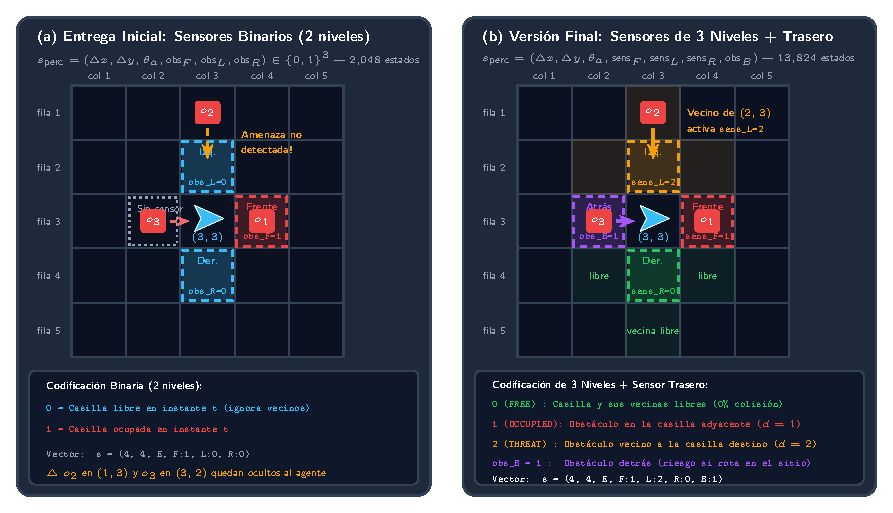
\includegraphics[width=0.78\textwidth]{fig_sensores_3niveles.pdf}
\caption{Comparación entre la percepción local de la entrega inicial y la ampliación a sensores de 3 niveles más sensor trasero para el agente en \((3,3)\) orientado al Este (\(\theta_a=1\)) con obstáculos en \((3,4)\), \((1,3)\) y \((3,2)\): (a) el modelo binario anterior codifica \(s=(4,4,E,1,0,0)\), dejando ocultos tanto la amenaza \(o_2\) en \((1,3)\) como el obstáculo trasero \(o_3\) en \((3,2)\); (b) el modelo ampliado codifica \(s=(4,4,E,1,2,0,1)\), distinguiendo casilla libre segura (\texttt{sens\_R=0}), ocupada (\texttt{sens\_F=1}), amenazada a un paso (\texttt{sens\_L=2}) y ocupada atrás (\texttt{obs\_B=1}).}
\label{fig:sensores_3niveles}
\end{figure}
    \item \textbf{Actualización del tamaño de la \(Q\)-tabla:}
    El vector de estado perceptual implementado es:
    \begin{equation}
        s_{\text{percepción}} = \big(\Delta x_{\text{meta}},\, \Delta y_{\text{meta}},\, \theta_a,\, \text{sens}_{\text{frente}},\, \text{sens}_{\text{izq}},\, \text{sens}_{\text{der}},\, \text{obs}_{\text{atrás}}\big)
    \end{equation}
    donde \(\Delta x_{\text{meta}} = 7 - x_a \in \{0,\dots,7\}\) y \(\Delta y_{\text{meta}} = 7 - y_a \in \{0,\dots,7\}\). El número total de estados perceptuales pasó de \(2{,}048\) a:
    \begin{equation}
        |\mathcal{S}_{\text{percepción}}| = 8 \times 8 \times 4 \times 3^3 \times 2 = 13{,}824 \text{ estados}
    \end{equation}
    lo que produce una \(Q\)-tabla de \(13{,}824 \times 3 = 41{,}472\) entradas.
    \item \textbf{Reglas de transición y entrenamiento mejoradas:}
    \begin{itemize}
        \item \emph{Distancia segura de aparición (\texttt{SAFE\_SPAWN\_DISTANCE = 3}):} los obstáculos se generan a distancia Manhattan \(\ge 3\) de \((0,0)\) y nunca ingresan a la celda meta \((7,7)\).
        \item \emph{Moldeo de recompensa (Reward Shaping) y prior físico:} durante el entrenamiento se emplea una señal moldeada \(R_{\text{train}} = R(s,a,s') + 2.0\big((\Delta x + \Delta y) - (\Delta x' + \Delta y')\big)\) e inicialización informada por la geometría y paridad del MDP (\texttt{compute\_physics\_prior}).
        \item \emph{Actualización simétrica en línea y tasa adaptativa:} cada transición actualiza simultáneamente el estado \((s,a)\) y su reflejo respecto a la diagonal principal del tablero, empleando una tasa de aprendizaje decreciente por conteo de visitas \(\alpha_{\text{eff}}(s,a) = \max\!\big(0.005, \frac{\alpha}{1 + 0.02 N(s,a)}\big)\) (Figura~\ref{fig:reglas_entrenamiento}).
    \end{itemize}
\end{enumerate}

\begin{figure}[ht!]
\centering
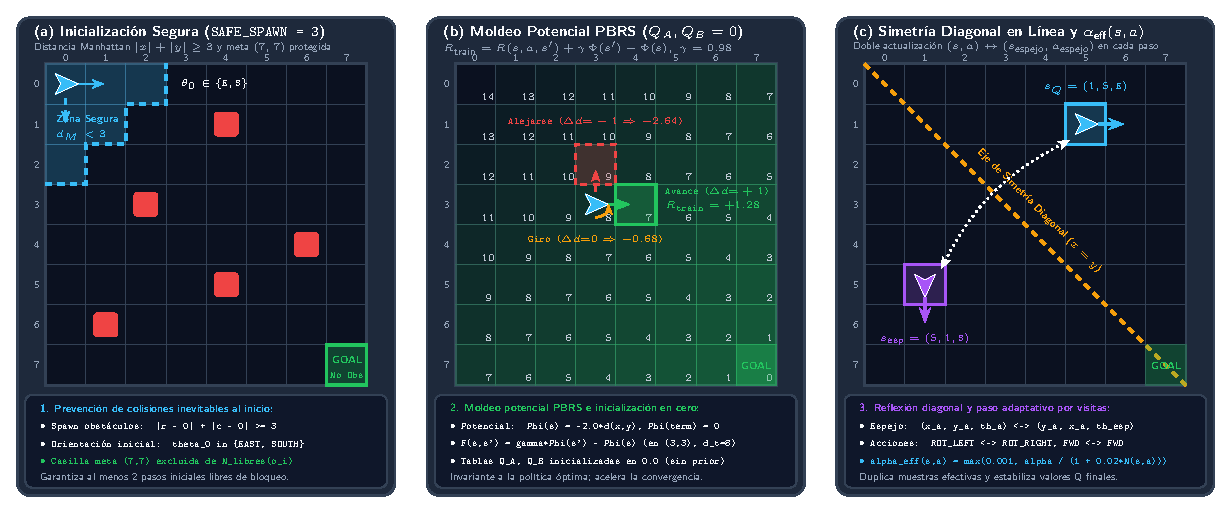
\includegraphics[width=0.80\textwidth]{fig_reglas_entrenamiento.pdf}
\caption{Esquema visual de las reglas de transición y entrenamiento mejoradas: (a) zona segura de aparición inicial (\texttt{SAFE\_SPAWN\_DISTANCE = 3}) alrededor de \((0,0)\) y exclusión de obstáculos en la meta \((7,7)\); (b) gradiente potencial Manhattan \(d(x,y)=(7-x)+(7-y)\) para el moldeo de recompensa \(R_{\text{train}}\) y prior físico de la \(Q\)-tabla; (c) reflexión diagonal en línea \((s,a) \leftrightarrow (s_{\text{espejo}}, a_{\text{espejo}})\) sobre el eje \(x=y\) y tasa de aprendizaje adaptativa \(\alpha_{\text{eff}}(s,a)\).}
\label{fig:reglas_entrenamiento}
\end{figure}

\begin{table}[h!]
\centering
\small
\renewcommand{\arraystretch}{1.18}
\caption{Resumen comparativo entre la definición de la entrega inicial y la implementación final.}
\vspace{0.15cm}
\begin{tabularx}{\textwidth}{@{}>{\raggedright\arraybackslash}p{3.2cm} >{\raggedright\arraybackslash}p{5.0cm} >{\raggedright\arraybackslash}X@{}}
\toprule
\textbf{Componente} & \textbf{Entrega Inicial} & \textbf{Implementación Final Reportada} \\ \midrule
Sensores locales & 3 sensores binarios (\(\{0,1\}^3\)): frente, izquierda, derecha. & 3 sensores de 3 niveles (\(\{0,1,2\}^3\): libre, ocupado, amenaza) + 1 sensor trasero binario (\(\{0,1\}\)). \\ \midrule
Estados perceptuales & \(8 \times 8 \times 4 \times 2^3 = 2{,}048\) estados. & \(8 \times 8 \times 4 \times 3^3 \times 2 = 13{,}824\) estados. \\ \midrule
Tamaño de la \(Q\)-tabla & \(2{,}048 \times 3 = 6{,}144\) entradas. & \(13{,}824 \times 3 = 41{,}472\) entradas. \\ \midrule
Dinámica de colisión & Coincidencia de casilla final (\(x'_a = x'_o\)). & Coincidencia de celda final y colisión frontal en arista intermedia por cruce simultáneo (\(x'_a = x_o \land x'_o = x_a\)). \\ \midrule
Persistencia y explotación & No especificada en código. & Guardado en disco (\texttt{q\_table.npy}) y carga en agente de explotación (\(\epsilon = 0.0\)). \\ \bottomrule
\end{tabularx}
\end{table}

\subsection{Conjunto de acciones (\(\mathcal{A}\))}
De acuerdo con la especificación del problema, el agente dispone de tres acciones discretas en todo estado no terminal (\(\mathcal{A} = \{a_0, a_1, a_2\}\)), ilustradas en la Figura~\ref{fig:acciones}:
\begin{itemize}[leftmargin=1.2cm]
    \item \textbf{\(a_0\) (\texttt{ACTION\_ROTATE\_LEFT}):} rota \(90^\circ\) a la izquierda sobre su propio eje sin cambiar de casilla: \(\theta'_a = (\theta_a - 1) \bmod 4\), \((x'_a, y'_a) = (x_a, y_a)\).
    \item \textbf{\(a_1\) (\texttt{ACTION\_ROTATE\_RIGHT}):} rota \(90^\circ\) a la derecha sobre su propio eje sin cambiar de casilla: \(\theta'_a = (\theta_a + 1) \bmod 4\), \((x'_a, y'_a) = (x_a, y_a)\).
    \item \textbf{\(a_2\) (\texttt{ACTION\_FORWARD}):} avanza una casilla en la dirección actual \(\theta_a\) si la casilla destino pertenece a \(\{0,\dots,7\}^2\); si intenta salir de los límites de la cuadrícula, choca contra la pared y permanece en \((x_a, y_a)\).
\end{itemize}

\begin{figure}[ht!]
\centering
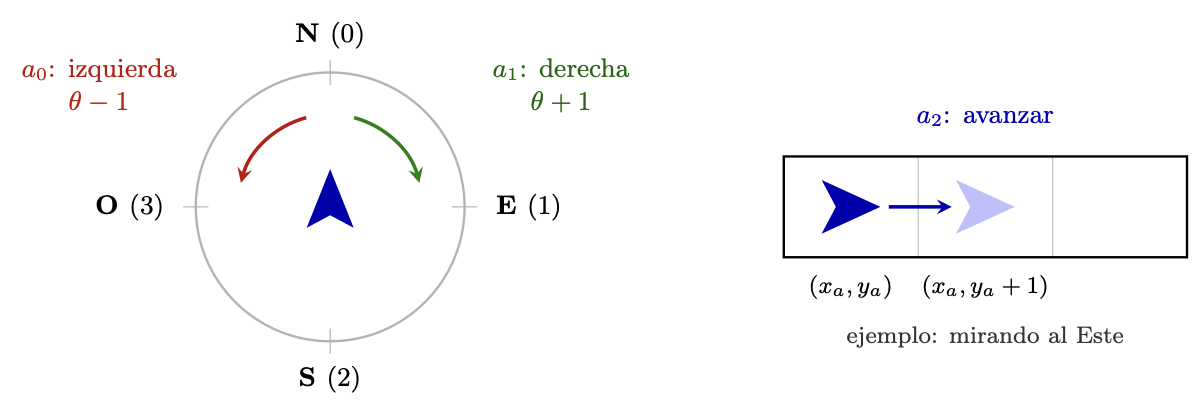
\includegraphics[width=0.50\textwidth]{fig_acciones.png}
\caption{Grados de libertad y conjunto de acciones del agente (\(\mathcal{A} = \{a_0, a_1, a_2\}\)).}
\label{fig:acciones}
\end{figure}

\subsection{Sistema de recompensas (\(R(s, a, s')\)) y dinámica de transición (\(P\))}
La función de recompensa del ambiente evalúa cada transición \((s, a, s')\) según cuatro eventos mutuamente excluyentes (Figura~\ref{fig:recompensas}):
\begin{equation}
    R(s, a, s') = 
    \begin{cases}
        \mathbf{+100.0} & \text{si } (x'_a, y'_a) = (7, 7) \quad \text{[Llegada a la meta]} \\
        \mathbf{-100.0} & \text{si } x'_a \in \mathcal{O}' \lor \exists\, i : (x'_a = x_{o_i} \land x'_{o_i} = x_a) \quad \text{[Colisión / cruce frontal]} \\
        \mathbf{-5.0}   & \text{si } a = a_2 \text{ y } (x'_a, y'_a) = (x_a, y_a) \quad \text{[Choque contra pared]} \\
        \mathbf{-1.0}   & \text{en cualquier otro paso no terminal (avance libre o rotación)}
    \end{cases}
\end{equation}

\begin{figure}[ht!]
\centering
\begin{minipage}[t]{0.48\textwidth}
\centering
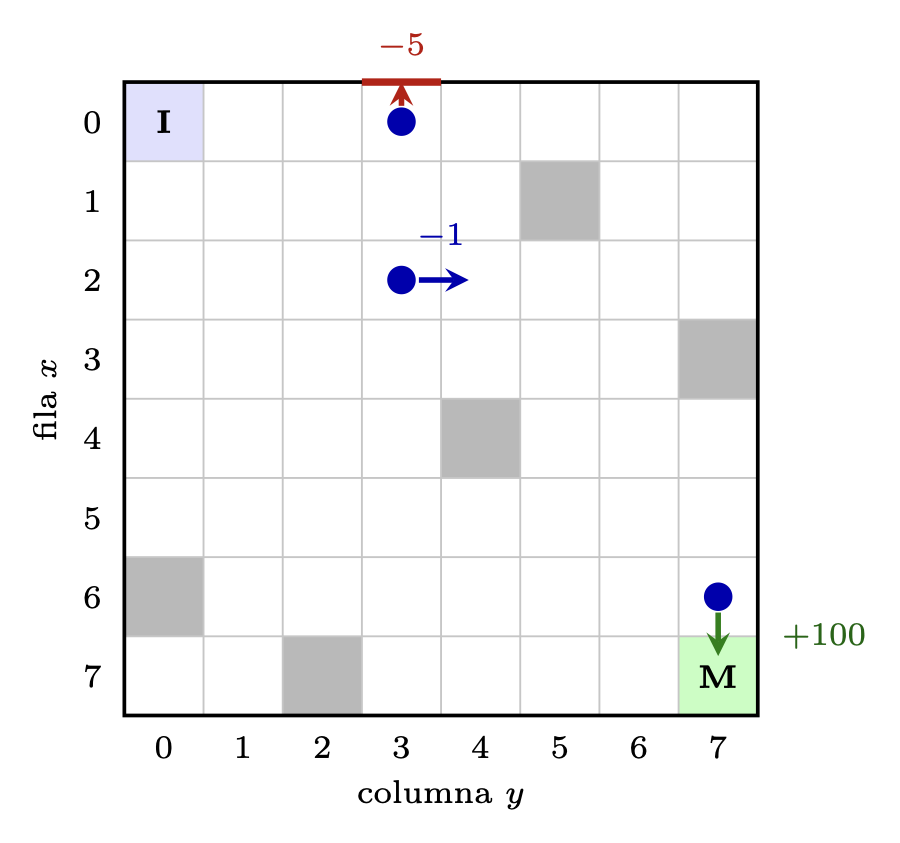
\includegraphics[width=0.92\textwidth]{fig_recompensas.png}
\caption{Ejemplos del sistema de recompensas \(R(s,a,s')\): llegada a la meta, colisión con obstáculo, choque contra pared y paso regular.}
\label{fig:recompensas}
\end{minipage}\hfill
\begin{minipage}[t]{0.48\textwidth}
\centering
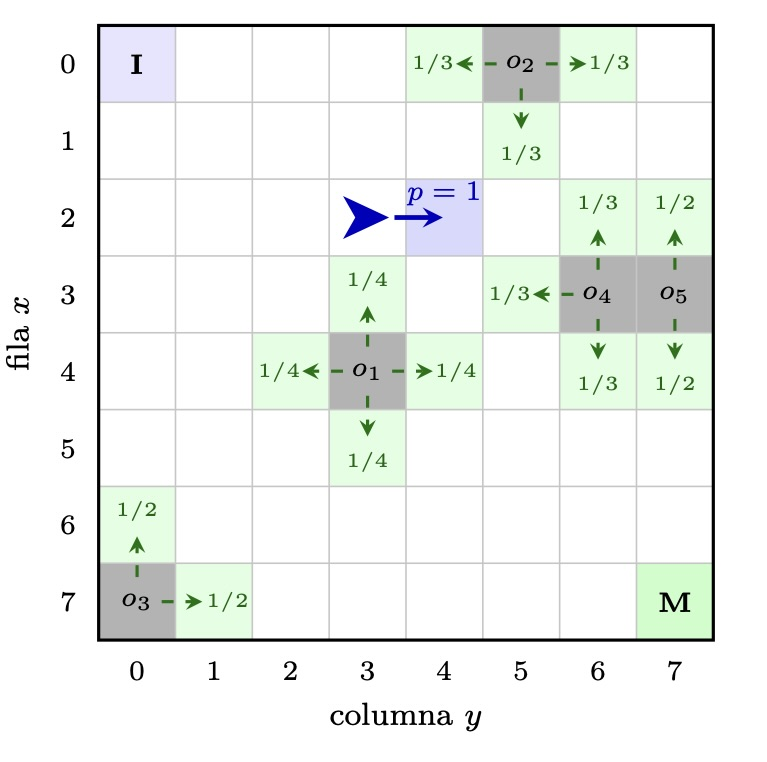
\includegraphics[width=0.92\textwidth]{fig_transicion.png}
\caption{Dinámica de transición simultánea del agente (determinista, \(p=1\)) y de los cinco obstáculos móviles (caminata aleatoria uniforme sobre las casillas vecinas libres).}
\label{fig:transicion}
\end{minipage}
\end{figure}

\section{Condiciones de Hardware/Software y Tiempos de Ejecución}
El entrenamiento, la serialización de la \(Q\)-tabla y las pruebas de validación se ejecutaron localmente bajo la configuración de hardware y software detallada en la Tabla~\ref{tab:hw_sw}.

\begin{table}[h!]
\centering
\small
\renewcommand{\arraystretch}{1.18}
\caption{Especificaciones de hardware, software e hiperparámetros de entrenamiento.}
\label{tab:hw_sw}
\vspace{0.15cm}
\begin{tabularx}{\textwidth}{@{}>{\raggedright\arraybackslash}p{4.0cm} >{\raggedright\arraybackslash}X@{}}
\toprule
\textbf{Parámetro / Recurso} & \textbf{Especificación} \\ \midrule
\textbf{Procesador (CPU)} & Apple M5 Pro (15 núcleos de CPU, arquitectura ARM64) \\
\textbf{Memoria RAM} & 24 GB de memoria unificada \\
\textbf{Sistema Operativo} & macOS 26.6.2 (Build 25G83) \\
\textbf{Lenguaje y Librerías} & Python 3, NumPy (\texttt{float64}), generación de reportes JSON y visualización HTML5 Canvas \\
\textbf{Hiperparámetros RL} & Episodios \(= 50{,}000\), máx.\ pasos/episodio \(= 200\), \(\alpha_0 = 0.08\) (adaptativo por visitas), \(\gamma = 0.98\), \(\epsilon_{\text{start}} = 1.0\), \(\epsilon_{\text{min}} = 0.01\), \(\epsilon_{\text{decay}} = 0.9995\), semilla (\texttt{seed}) \(= 42\) \\ \bottomrule
\end{tabularx}
\end{table}

La Tabla~\ref{tab:tiempos} reporta el desglose de los tiempos de ejecución medidos en la última corrida del sistema. El entrenamiento completo de \(50{,}000\) episodios (aproximadamente \(1.06 \times 10^6\) pasos de interacción y \(2.13 \times 10^6\) actualizaciones de la \(Q\)-tabla, incluyendo las actualizaciones simétricas en línea) finaliza en \(14.8\text{ segundos}\), con una velocidad media de \(\sim 3{,}385\text{ episodios/segundo}\).

\begin{table}[h!]
\centering
\small
\renewcommand{\arraystretch}{1.18}
\caption{Tiempos de ejecución por etapa del flujo de entrenamiento y evaluación.}
\label{tab:tiempos}
\vspace{0.15cm}
\begin{tabularx}{\textwidth}{@{}>{\raggedright\arraybackslash}p{6.5cm} c >{\raggedright\arraybackslash}X@{}}
\toprule
\textbf{Etapa del Proceso} & \textbf{Tiempo (s)} & \textbf{Detalle de Operación} \\ \midrule
Inicialización del prior físico & \(0.02\text{ s}\) & Cálculo de valores iniciales sobre las \(41{,}472\) entradas \\
Entrenamiento \(Q\)-Learning (\(50{,}000\) ep.) y simetrización & \(14.77\text{ s}\) & \(\sim 3{,}385\text{ ep./s}\) con actualización dual \((s,a)\) y espejo; fusión ponderada por visitas \\
Guardado y carga (\texttt{q\_table.npy}) & \(0.02\text{ s}\) & Escritura en disco y carga en agente de explotación \\
Evaluación en \(500\) episodios (\texttt{main.py}) & \(0.09\text{ s}\) & Explotación pura (\(\epsilon = 0.0\)) desde archivo cargado \\
Evaluación en \(1{,}000\) ep.\ + 20 sims (\texttt{test\_simulations.py}) & \(0.20\text{ s}\) & Validación estadística y exportación HTML/JSON \\ \midrule
\textbf{Tiempo total del pipeline completo} & \(\mathbf{15.10\text{ s}}\) & Entrenamiento, validación y generación de reportes \\ \bottomrule
\end{tabularx}
\end{table}

\section{Resultados Experimentales de Validación}
Una vez finalizado el entrenamiento, la memoria del agente se grabó en el archivo \texttt{q\_table.npy} (\(41{,}472\) entradas) y se cargó en una nueva instancia de \texttt{QLearningAgent} con \(\epsilon = 0.0\) para evaluar la política aprendida sin exploración aleatoria. La Tabla~\ref{tab:metricas} resume el desempeño obtenido frente a la línea base inicial y bajo las dos modalidades de movimiento del ambiente.

\begin{table}[ht!]
\centering
\small
\renewcommand{\arraystretch}{1.2}
\caption{Resultados cuantitativos de evaluación de la política cargada desde \texttt{q\_table.npy}.}
\label{tab:metricas}
\vspace{0.15cm}
\begin{tabularx}{\textwidth}{@{}>{\raggedright\arraybackslash}X c c c c c@{}}
\toprule
\textbf{Configuración Evaluada} & \textbf{Éxito} & \textbf{Colisión} & \textbf{Recompensa Media} & \textbf{Pasos} & \textbf{Pared} \\ \midrule
Línea base previa (Sin penalizar cruce frontal, \(1{,}000\) ep.) & \(75.8\%\) & \(24.2\%\) & \(+34.25 \pm 82.99\) & \(18.3\) & \(0.00\) \\
\textbf{Agente mejorado con colisión frontal (Simultáneo, \(500\) ep.)} & \(\mathbf{56.2\%}\) & \(\mathbf{43.8\%}\) & \(\mathbf{-3.26 \pm 95.67}\) & \(\mathbf{16.7}\) & \(\mathbf{0.00}\) \\
\textbf{Agente mejorado con colisión frontal (Simultáneo, \(1{,}000\) ep.)} & \(\mathbf{54.5\%}\) & \(\mathbf{45.5\%}\) & \(\mathbf{-6.35 \pm 95.88}\) & \(\mathbf{16.3}\) & \(\mathbf{0.00}\) \\
Agente mejorado (Muestra 20 sims grabadas) & \(\mathbf{60.0\%}\) & \(40.0\%\) & \(+5.85 \pm 94.75\) & \(15.2\) & \(0.00\) \\
Agente mejorado (Modo Secuencial, \(1{,}000\) ep.) & \(\mathbf{100.0\%}\) & \(\mathbf{0.0\%}\) & \(\mathbf{+84.06 \pm 2.75}\) & \(\mathbf{16.9}\) & \(\mathbf{0.00}\) \\ \bottomrule
\end{tabularx}
\end{table}

En las 20 simulaciones grabadas (\texttt{simulations\_report.json} y \texttt{simulations\_animation.html}), el agente alcanzó la meta en 12 de los 20 episodios (\(60.0\%\)) y en 7 de los primeros 10 episodios (\(70.0\%\)), destacando trayectorias óptimas de 15 pasos con recompensa \(+86.0\) (\texttt{Sim \#8, \#10}) y maniobras evasivas exitosas (\texttt{Sim \#1, \#3, \#4, \#6, \#7, \#11, \#13, \#14, \#19, \#20}). La Figura~\ref{fig:sim_transiciones} ilustra cuatro estados de transición representativos de la dinámica del entorno, mostrando la activación de los sensores locales de 3 niveles, la maniobra de giro ante amenaza (\(\text{sens}_{\text{frente}}=2\)), el diagnóstico de la regla física de colisión frontal por cruce simultáneo (\(x'_a = x_o \land x'_o = x_a \implies \text{Colisión}\)) sobre una casilla ocupada (\(\text{sens}_{\text{frente}}=1\)) y la llegada a la meta \((7,7)\).

\begin{figure}[ht!]
\centering
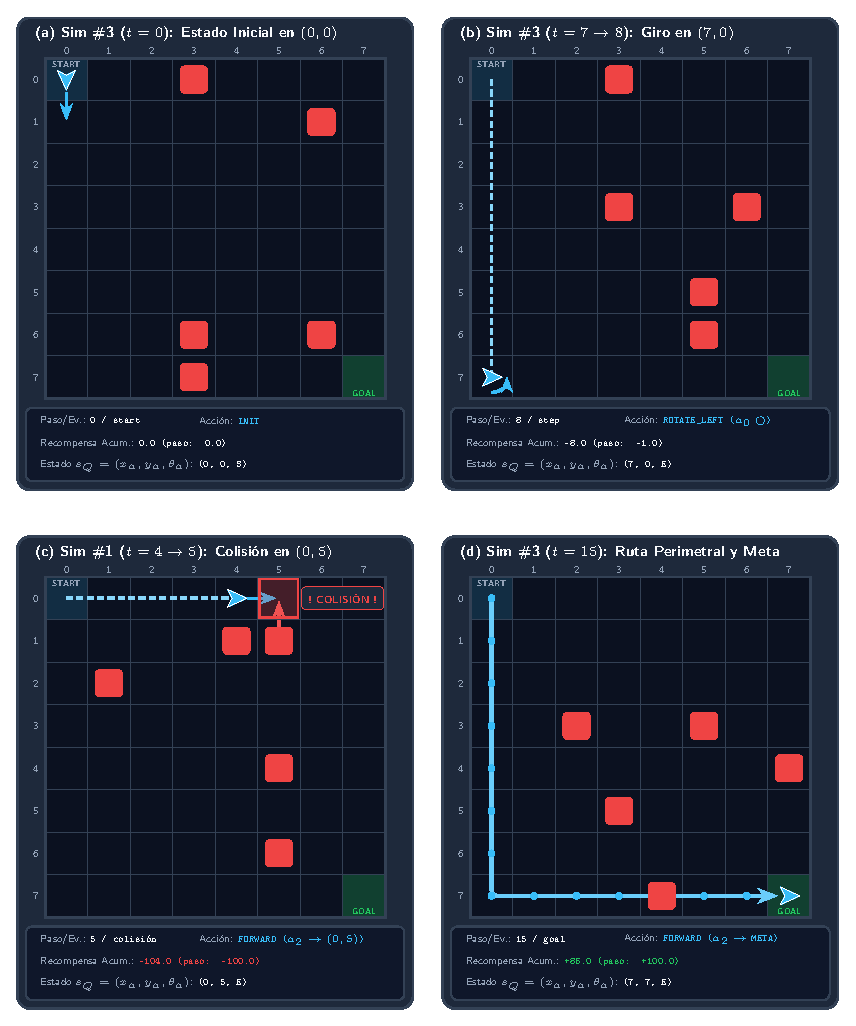
\includegraphics[width=0.78\textwidth]{fig_simulacion_transiciones.pdf}
\caption{Secuencia de estados de transición del entorno: (a) estado inicial en \((0,0)\) con sensores libres; (b) detección de amenaza (\texttt{F:2, L:2}) en \((1,0)\) y giro evasivo \(a_0\) hacia el Este; (c) colisión frontal por cruce simultáneo de posiciones (\(x'_a = x_o \land x'_o = x_a\)) al intentar avanzar sobre una casilla ocupada (\texttt{F:1}), penalizada con \(R=-100\); (d) trayectoria óptima completa hasta la meta \((7,7)\) ejecutando la política aprendida.}
\label{fig:sim_transiciones}
\end{figure}
\section{Comportamiento Esperado vs.\ Comportamiento No Esperado Observado}

\subsection{Comportamiento esperado del agente}
Durante la explotación de la \(Q\)-tabla entrenada se observaron tres conductas consistentes con el diseño del MDP. En primer lugar, cuando el corredor perimetral está despejado, el agente sigue la ruta mínima de 15 pasos (recompensa \(+86.0\)): avanza 7 casillas en su dirección inicial (\(\text{Sur}\) hasta \((7,0)\) o \(\text{Este}\) hasta \((0,7)\)), ejecuta una única rotación de \(90^\circ\) en la esquina y avanza 7 casillas adicionales hasta \((7,7)\). Además de minimizar los giros, el perímetro presenta menor densidad estacionaria de obstáculos; en una caminata aleatoria uniforme sobre un grafo no dirigido, la distribución estacionaria es proporcional al grado del nodo (\(\pi(v) \propto \deg(v)\)), por lo que las celdas interiores (\(\deg = 4\)) concentran un \(33\%\) más de tráfico que los bordes (\(\deg = 3\)) y el doble que las esquinas (\(\deg = 2\)).

En segundo lugar, se obtuvo la eliminación total de choques contra las paredes (\texttt{mean\_wall\_hits = 0.0}), dado que el agente identifica los bordes de la cuadrícula a partir de \((\Delta x_{\text{meta}}, \Delta y_{\text{meta}}, \theta_a)\) y evita avanzar fuera del tablero o girar hacia un muro exterior. Por último, cuando el sensor frontal detecta amenaza (\(\text{sens}_{\text{frente}} = 2\)) sin obstáculos adyacentes (\(\text{adj\_count} = 0\)), el agente utiliza la rotación como maniobra de espera sin riesgo inmediato para cambiar la paridad en el grafo bipartito del tablero, permitiendo que el obstáculo despeje la ruta o desviándose por filas y columnas interiores (observado en \texttt{Sim \#1} y \texttt{Sim \#3}).

\subsection{Comportamiento no esperado observado y su diagnóstico}
Durante el análisis de las simulaciones interactivas se identificaron tres fenómenos que explican las fallas iniciales y el límite de desempeño del modo simultáneo:

\begin{enumerate}[leftmargin=1.2cm]
    \item \textbf{Colisión frontal por cruce simultáneo de posiciones (\(x'_a = x_o \land x'_o = x_a\)):}
    En las primeras versiones del ambiente, cuando el agente avanzaba hacia una casilla ocupada (\(\text{sens}_{\text{frente}} = 1\)) y el obstáculo se desplazaba al mismo tiempo hacia la celda previa del agente, el comprobador de colisiones evaluaba únicamente la coincidencia final (\(x'_a = x'_o\)). Al intercambiar posiciones sin compartir celda final, la transición se registraba como segura. Físicamente, este intercambio equivale a un cruce frontal en la arista intermedia, por lo que se incorporó la verificación \texttt{crossed\_head\_on} en \texttt{environment.py}:
    \begin{equation}
    \text{Colisión} \iff (x'_a \in \mathcal{O}') \lor \exists o \in \mathcal{O}: (x'_a = x_o \land x'_o = x_a)
    \end{equation}
    Al penalizar este cruce con \(R = -100\), avanzar hacia \(\text{sens}_{\text{frente}} = 1\) conlleva un riesgo de colisión entre \(25\%\) y \(50\%\), lo que lleva a la \(Q\)-tabla a favorecer maniobras evasivas o giros preventivos.

    \item \textbf{Borrado de penalizaciones negativas durante la simetrización con \(\max(\cdot)\):}
    Inicialmente, la función \texttt{symmetrize\_q\_table} aplicaba \(\max\big(Q(s,a), Q(s_{\text{m}}, a_{\text{m}})\big)\) al finalizar el entrenamiento, provocando acciones suicidas en estados poco frecuentes. Si un estado peligroso \(s\) tenía valores aprendidos negativos (p.\ ej., \(-15.0\) para esquivar y \(-90.0\) para chocar), pero su espejo \(s_{\text{espejo}}\) no había sido visitado (\(Q = 0.0\)), el operador \(\max(\cdot, 0.0)\) sobrescribía ambas entradas con \(0.0\). Esto se corrigió registrando la matriz de visitas \texttt{visit\_counts} y realizando actualizaciones simétricas en línea en cada paso.

    \item \textbf{Límite estocástico ante 5 obstáculos en movimiento simultáneo:}
    Al penalizar el cruce frontal y las colisiones simultáneas, la tasa de éxito en modo simultáneo se sitúa en \(\approx 55\%\text{--}60\%\) sobre \(1{,}000\) episodios. En cada paso de tiempo, el agente solo puede permanecer en su celda actual (si rota) o avanzar a la celda frontal. Cuando un obstáculo se encuentra adyacente o a 2 casillas en ruta de convergencia, ambas decisiones presentan una probabilidad positiva de colisión (\(P \ge 0.25\)). Con 5 obstáculos en una cuadrícula \(8 \times 8\), el agente enfrenta entre 1 y 3 cruces forzados por trayectoria, lo que acota la supervivencia en 15 pasos cerca de \((1 - 0.25)^2 \approx 56.2\%\), en concordancia con el desempeño empírico observado (\(54.5\%\text{--}56.2\%\)).
\end{enumerate}

\section{Posible Mejora: Acción Compuesta de Rotación y Avance Simultáneo}

Una limitación estructural del MDP actual es el desacoplamiento temporal entre girar y avanzar. Cuando el agente ejecuta una rotación (\(a_0\) o \(a_1\)), permanece inmóvil en \((x_a, y_a)\) durante ese paso de tiempo, quedando expuesto a que un obstáculo adyacente invada su celda.

Para reducir las colisiones en modo simultáneo, se propone como trabajo futuro extender el espacio de acciones a tuplas coordinadas \(a = (\Delta\theta, \text{avance})\). En lugar de requerir turnos independientes para orientarse y avanzar, el agente combinaría giros relativos (\(0^\circ, \pm 90^\circ, 180^\circ\)) con el desplazamiento de una casilla en la nueva dirección, manteniendo la rotación de \(360^\circ\) en el sitio como espera activa cuando todas las celdas vecinas estén ocupadas o amenazadas. De este modo, ante un bloqueo frontal, el agente podría desviarse lateralmente o retroceder en una única transición sin quedar inmovilizado.

Para evitar giros innecesarios, la función de recompensa conservaría una penalización desglosada por componente físico:
\begin{equation}
R_{\text{paso}}(a) = R_{\text{traslación}} + R_{\text{rotación}}(\Delta\theta) = -1.0 - k_{\text{rot}} \left(\frac{|\Delta\theta|}{90^\circ}\right)
\end{equation}
donde cada cuarto de vuelta añade un costo individual (p.\ ej., \(k_{\text{rot}} = 0.5\) o \(1.0\)). Así, avanzar de frente costaría \(-1.0\), rotar \(90^\circ\) y avanzar \(-2.0\), girar \(180^\circ\) y retroceder \(-3.0\), y rotar \(360^\circ\) en el sitio \(-5.0\). Esta formulación preserva el incentivo hacia la ruta mínima, pero permite que la política asuma el costo de girar y desplazarse cuando avanzar de frente implica riesgo de colisión (\(-100.0\)).

Al disponer de cuatro direcciones de desplazamiento inmediato en lugar de una sola, disminuye la probabilidad de quedar atrapado en estados sin salida segura frente al movimiento aleatorio de los cinco obstáculos. Aunque su cuantificación exacta requiere implementación y validación experimental, se espera que esta extensión reduzca la brecha de desempeño observada entre el modo simultáneo y el modo secuencial sin perder la interpretabilidad tabular de la \(Q\)-tabla.

\end{document}
